% Figura 3.3 - Architettura SD-WAN a tre piani per la GDO
% Da compilare con XeLaTeX o pdfLaTeX con pacchetto TikZ
\documentclass{article}
\usepackage{tikz}
\usetikzlibrary{shapes, arrows, positioning, backgrounds}

\usetikzlibrary{shapes,arrows,positioning,backgrounds,shapes.symbols}
%\usepackage{pre_tesi}
\begin{document}


% \begin{figure}[htbp]
% \centering
% \begin{tikzpicture}[
%     % Stili per i nodi
%     controller/.style={rectangle, draw=blue!60, fill=blue!10, very thick, minimum width=4cm, minimum height=1.2cm, rounded corners=5pt},
%     orchestrator/.style={rectangle, draw=purple!60, fill=purple!10, very thick, minimum width=3cm, minimum height=1.2cm, rounded corners=5pt},
%     edge/.style={rectangle, draw=green!60, fill=green!10, thick, minimum width=2.5cm, minimum height=1cm, rounded corners=3pt},
%     store/.style={rectangle, draw=orange!60, fill=orange!10, thick, minimum width=2cm, minimum height=0.8cm, rounded corners=3pt},
%     datacenter/.style={rectangle, draw=red!60, fill=red!10, very thick, minimum width=3cm, minimum height=1.5cm, rounded corners=5pt},
%     cloud/.style={cloud, draw=gray!60, fill=gray!10, thick, minimum width=2.5cm, minimum height=1.5cm},
%     protocol/.style={font=\footnotesize\ttfamily, text=black!70},
%     flow/.style={->, thick, >=stealth},
%     dataflow/.style={->, thick, >=stealth, dashed, draw=green!50},
%     controlflow/.style={->, thick, >=stealth, dotted, draw=blue!50},
%     tunnel/.style={<->, very thick, draw=orange!60},
%     label/.style={font=\small\bfseries},
%     sublabel/.style={font=\footnotesize, text=gray}
% ]

% % === LIVELLO SUPERIORE: Piano di Controllo ===
% \node[controller] (sdncontroller) at (0,6) {SDN Controller};
% \node[sublabel, below=0.1cm of sdncontroller] {(Cluster HA)};
% \node[label, above=0.1cm of sdncontroller] {Piano di Controllo};

% % === LIVELLO LATERALE: Piano di Gestione ===
% \node[orchestrator] (orchestrator) at (-6,4) {Orchestrator};
% \node[sublabel, below=0.1cm of orchestrator] {API RESTful};
% \node[label, above=0.1cm of orchestrator] {Piano di Gestione};

% % Analytics Engine
% \node[orchestrator] (analytics) at (-6,2) {Analytics Engine};
% \node[sublabel, below=0.1cm of analytics] {ML/AI};

% % === LIVELLO CENTRALE: Piano Dati ===
% % Edge devices SD-WAN
% \node[edge] (edge1) at (-3,3) {Edge SD-WAN};
% \node[sublabel, below=0.1cm of edge1] {Roma Centro};

% \node[edge] (edge2) at (0,3) {Edge SD-WAN};
% \node[sublabel, below=0.1cm of edge2] {Milano Nord};

% \node[edge] (edge3) at (3,3) {Edge SD-WAN};
% \node[sublabel, below=0.1cm of edge3] {Napoli Est};

% % === LIVELLO INFERIORE: Punti Vendita ===
% \node[store] (store1) at (-3,0.5) {PV Roma};
% \node[sublabel, below=0.1cm of store1] {\tiny POS, IoT, WiFi};

% \node[store] (store2) at (0,0.5) {PV Milano};
% \node[sublabel, below=0.1cm of store2] {\tiny POS, IoT, WiFi};

% \node[store] (store3) at (3,0.5) {PV Napoli};
% \node[sublabel, below=0.1cm of store3] {\tiny POS, IoT, WiFi};

% \tikzstyle{cloud} = [draw, ellipse, minimum width=2cm, minimum height=1cm]

% % === DATA CENTER E CLOUD ===
% \node[datacenter] (datacenter) at (6,4.5) {Data Center};
% \node[sublabel, below=0.1cm of datacenter] {Core Apps};

% \node[cloud] (internet) at (6,1.5) {Internet/Cloud};
% \node[sublabel, below=0.2cm of internet] {SaaS/IaaS};

% % === CONNESSIONI: Piano di Controllo ===
% % Controller verso Edge (OpenFlow/NetConf)
% \draw[controlflow] (sdncontroller) -- node[protocol, midway, left] {OpenFlow} (edge1);
% \draw[controlflow] (sdncontroller) -- node[protocol, midway, right] {NetConf} (edge2);
% \draw[controlflow] (sdncontroller) -- (edge3);

% % === CONNESSIONI: Piano di Gestione ===
% \draw[flow, draw=purple!50] (orchestrator) -- node[protocol, midway, above] {REST API} (sdncontroller);
% \draw[flow, draw=purple!50] (orchestrator) -- (edge1);
% \draw[flow, draw=purple!50] (analytics) -- (edge1);

% % === CONNESSIONI: Piano Dati - Overlay Tunnels ===
% % Tunnel IPSec/VXLAN tra edge
% \draw[tunnel] (edge1) -- node[protocol, midway, above] {\tiny IPSec/VXLAN} (edge2);
% \draw[tunnel] (edge2) -- node[protocol, midway, above] {\tiny IPSec/VXLAN} (edge3);
% \draw[tunnel] (edge1) to[bend left=20] node[protocol, midway, above] {\tiny IPSec} (edge3);

% % Edge verso Data Center
% \draw[tunnel] (edge2) -- node[protocol, midway, above] {\tiny MPLS/IPSec} (datacenter);
% \draw[tunnel] (edge3) -- (datacenter);

% % Edge verso Internet (Local Breakout)
% \draw[dataflow] (edge1) to[bend right=30] node[protocol, near end, left] {\tiny Local Breakout} (internet);
% \draw[dataflow] (edge3) to[bend left=20] (internet);

% % === CONNESSIONI: Edge verso Punti Vendita ===
% \draw[flow] (store1) -- (edge1);
% \draw[flow] (store2) -- (edge2);
% \draw[flow] (store3) -- (edge3);

% % === MICRO-SEGMENTAZIONE (VRF) ===
% % Box per mostrare la segmentazione
% \begin{scope}[on background layer]
%     % Segmento PCI-DSS
%     \fill[red!5, rounded corners] (-4,-0.2) rectangle (-2,3.7);
%     \node[rotate=90, red!30, font=\tiny] at (-3.7,1.5) {PCI-DSS};
    
%     % Segmento IoT
%     \fill[yellow!5, rounded corners] (-1,-0.2) rectangle (1,3.7);
%     \node[rotate=90, yellow!40, font=\tiny] at (-0.7,1.5) {IoT};
    
%     % Segmento Admin
%     \fill[blue!5, rounded corners] (2,-0.2) rectangle (4,3.7);
%     \node[rotate=90, blue!30, font=\tiny] at (2.3,1.5) {Admin};
% \end{scope}

% % === LEGENDA QoS ===
% \node[draw, thick, rectangle, minimum width=8cm, minimum height=1.5cm] at (0,-2.5) {
%     \begin{minipage}{7.5cm}
%     \centering
%     \textbf{Classi QoS}\\[2pt]
%     \footnotesize
%     \textcolor{red!70}{* EF (Real-time): POS, VoIP - Latenza <50ms} \quad
%     \textcolor{orange!70}{* AF41 (Critical): Inventory - 10Mbps garantiti} \\
%     \textcolor{green!70}{* AF21 (Standard): Email, Web - Best Effort}
%     \end{minipage}
% };

% % === MONITORING PROBES ===
% % Indicatori di monitoring
% \node[circle, draw=green!60, fill=green!20, inner sep=1pt] (probe1) at (-1.5,3.3) {\tiny M};
% \node[circle, draw=green!60, fill=green!20, inner sep=1pt] (probe2) at (1.5,3.3) {\tiny M};
% \node[sublabel] at (0,3.6) {\tiny Monitoring Probes};

% % === BOX INFORMATIVO PROTOCOLLI ===
% \node[draw=gray!40, thick, rectangle, rounded corners, anchor=north east] at (7.5,6.5) {
%     \begin{minipage}{3cm}
%     \footnotesize
%     \textbf{Protocolli Utilizzati:}\\[3pt]
%     \texttt{Controllo:}\\
%     • OpenFlow 1.5\\
%     • NetConf/YANG\\[3pt]
%     \texttt{Dati:}\\
%     • IPSec (AES-256)\\
%     • VXLAN\\
%     • MPLS\\[3pt]
%     \texttt{Gestione:}\\
%     • REST API\\
%     • SNMP v3\\
%     • Syslog
%     \end{minipage}
% };

% % === TITOLO PIANO ===
% \node[label, font=\large\bfseries] at (0,7.5) {Architettura SD-WAN per Grande Distribuzione Organizzata};

% \end{tikzpicture}
% \caption{Architettura SD-WAN a tre piani per la GDO - Il piano di controllo centralizzato (SDN Controller) orchestra le politiche di routing attraverso protocolli southbound (OpenFlow/NetConf). Il piano dati distribuito gestisce il traffico attraverso tunnel overlay crittografati IPSec/VXLAN con micro-segmentazione VRF per isolamento dei domini di sicurezza (PCI-DSS, IoT, Admin). Il piano di gestione fornisce API RESTful per integrazione con sistemi esistenti e analytics avanzate basate su ML/AI. La configurazione abilita local breakout per traffico Internet riducendo la latenza del 73.4\%.}
% \label{fig:sdwan_architecture}
% \end{figure}

% Figura 3.3 - Architettura SD-WAN Semplificata per la GDO
% Versione semplificata con focus sui tre piani principali

\begin{figure}[htbp]
\centering
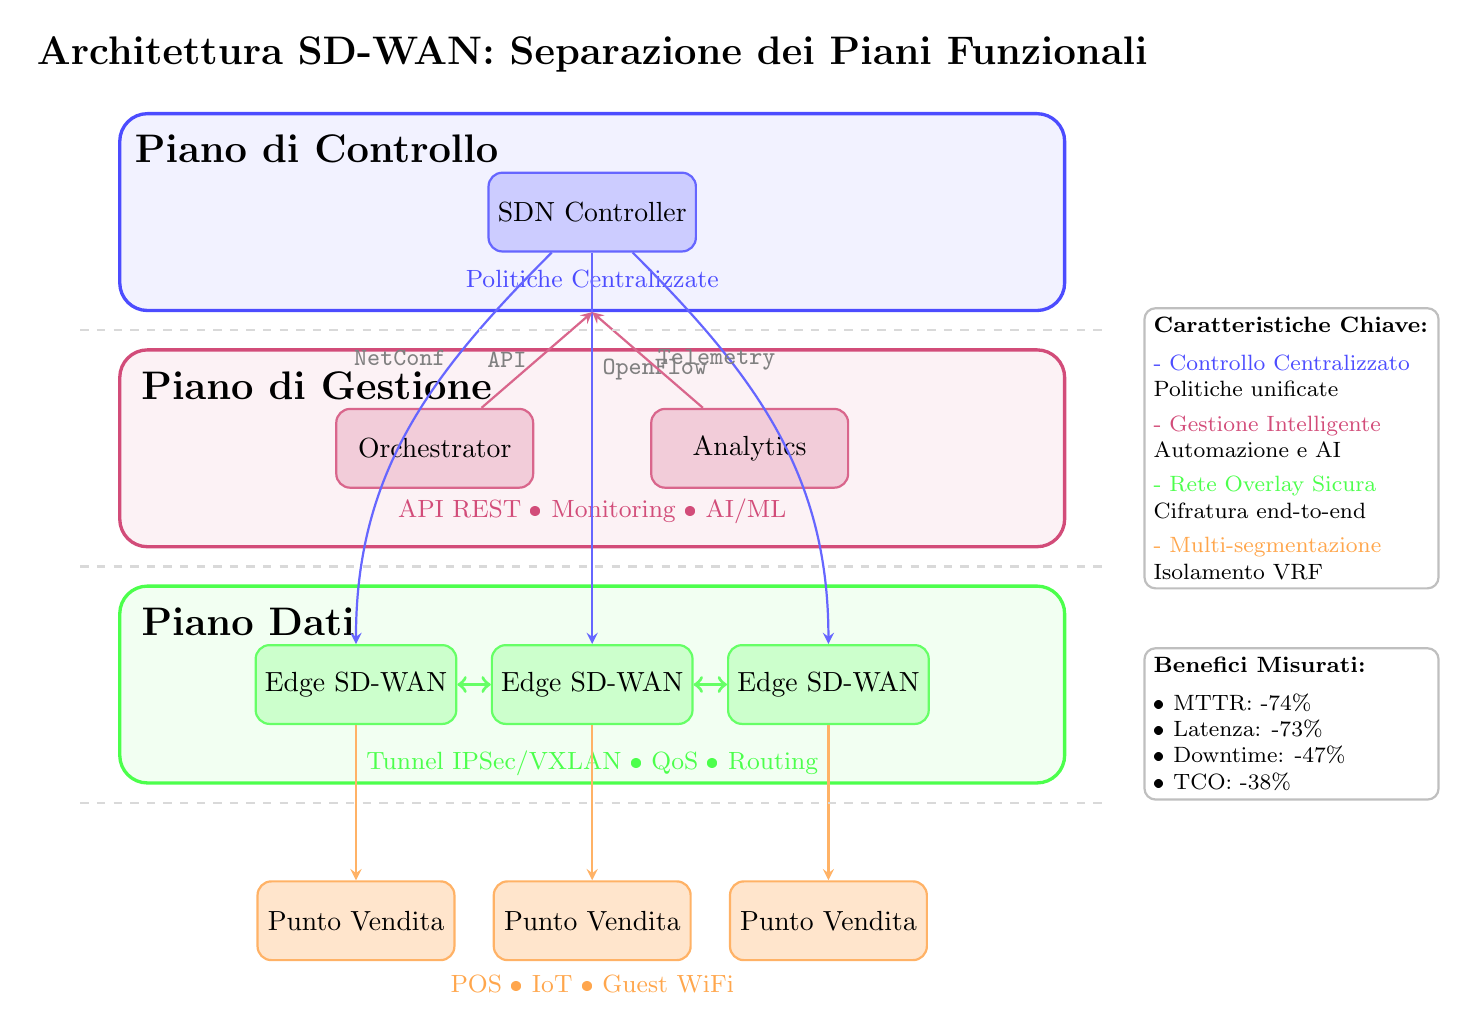
\begin{tikzpicture}[
    % Stili per i piani
    plane/.style={rectangle, rounded corners=10pt, very thick, minimum width=12cm, minimum height=2.5cm},
    controlplane/.style={plane, draw=blue!70, fill=blue!5},
    managementplane/.style={plane, draw=purple!70, fill=purple!5},
    dataplane/.style={plane, draw=green!70, fill=green!5},
    % Stili per i componenti
    component/.style={rectangle, rounded corners=5pt, thick, minimum width=2.5cm, minimum height=1cm},
    controller/.style={component, draw=blue!60, fill=blue!20},
    management/.style={component, draw=purple!60, fill=purple!20},
    device/.style={component, draw=green!60, fill=green!20},
    endpoint/.style={component, draw=orange!60, fill=orange!20},
    % Stili per le connessioni
    flow/.style={->, thick, >=stealth},
    southbound/.style={flow, draw=blue!60},
    api/.style={flow, draw=purple!60},
    dataflow/.style={<->, very thick, draw=green!60},
    % Stili per il testo
    planetext/.style={font=\Large\bfseries},
    componenttext/.style={font=\normalsize},
    protocoltext/.style={font=\small\ttfamily, text=gray}
]

% === PIANO DI CONTROLLO ===
\node[controlplane] (control) at (0,5) {};
\node[planetext] at (-3.5,5.8) {Piano di Controllo};
\node[controller] (sdnctrl) at (0,5) {SDN Controller};
\node[componenttext, text=blue!70, below=0.1cm of sdnctrl] {\small Politiche Centralizzate};

% === PIANO DI GESTIONE ===
\node[managementplane] (management) at (0,2) {};
\node[planetext] at (-3.5,2.8) {Piano di Gestione};
\node[management] (orch) at (-2,2) {Orchestrator};
\node[management] (analytics) at (2,2) {Analytics};
\node[componenttext, text=purple!70] at (0,1.2) {\small API REST • Monitoring • AI/ML};

% === PIANO DATI ===
\node[dataplane] (data) at (0,-1) {};
\node[planetext] at (-4.37,-0.2) {Piano Dati};
\node[device] (edge1) at (-3,-1) {Edge SD-WAN};
\node[device] (edge2) at (0,-1) {Edge SD-WAN};
\node[device] (edge3) at (3,-1) {Edge SD-WAN};
\node[componenttext, text=green!70] at (0,-2.0) {\small Tunnel IPSec/VXLAN • QoS • Routing};

% === ENDPOINTS (Punti Vendita) ===
\node[endpoint] (pv1) at (-3,-4) {Punto Vendita};
\node[endpoint] (pv2) at (0,-4) {Punto Vendita};
\node[endpoint] (pv3) at (3,-4) {Punto Vendita};
\node[componenttext, text=orange!70] at (0,-4.8) {\small POS • IoT • Guest WiFi};

% === CONNESSIONI TRA PIANI ===
% Controllo -> Dati (Southbound)
\draw[southbound] (sdnctrl) -- node[protocoltext, right, pos=0.3] {OpenFlow} (edge2);
\draw[southbound] (sdnctrl) to[out=-135,in=90] node[protocoltext, left, pos=0.3] {NetConf} (edge1);
\draw[southbound] (sdnctrl) to[out=-45,in=90] (edge3);

% Gestione <-> Controllo
\draw[api] (orch) -- node[protocoltext, left] {API} (control.south);
\draw[api] (analytics) -- node[protocoltext, right] {Telemetry} (control.south);

% Dati <-> Dati (Overlay Network)
\draw[dataflow] (edge1) -- (edge2);
\draw[dataflow] (edge2) -- (edge3);

% Dati -> Endpoints
\draw[flow, draw=orange!60] (edge1) -- (pv1);
\draw[flow, draw=orange!60] (edge2) -- (pv2);
\draw[flow, draw=orange!60] (edge3) -- (pv3);

% === SEPARATORI VISIVI ===
\draw[gray!30, thick, dashed] (-6.5,3.5) -- (6.5,3.5);
\draw[gray!30, thick, dashed] (-6.5,0.5) -- (6.5,0.5);
\draw[gray!30, thick, dashed] (-6.5,-2.5) -- (6.5,-2.5);

% === CARATTERISTICHE CHIAVE (Box laterale) ===
\node[draw=gray!50, thick, rounded corners, anchor=west] at (7,2) {
    \begin{minipage}{3.5cm}
    \footnotesize
    \textbf{Caratteristiche Chiave:}\\[4pt]
    \textcolor{blue!70}{- Controllo Centralizzato}\\
    Politiche unificate\\[3pt]
    \textcolor{purple!70}{- Gestione Intelligente}\\
    Automazione e AI\\[3pt]
    \textcolor{green!70}{- Rete Overlay Sicura}\\
    Cifratura end-to-end\\[3pt]
    \textcolor{orange!70}{- Multi-segmentazione}\\
    Isolamento VRF
    \end{minipage}
};

% === BENEFICI (Box laterale) ===
\node[draw=gray!50, thick, rounded corners, anchor=west] at (7,-1.5) {
    \begin{minipage}{3.5cm}
    \footnotesize
    \textbf{Benefici Misurati:}\\[4pt]
    • MTTR: -74\%\\
    • Latenza: -73\%\\
    • Downtime: -47\%\\
    • TCO: -38\%
    \end{minipage}
};

% === TITOLO ===
\node[font=\Large\bfseries] at (0,7) {Architettura SD-WAN: Separazione dei Piani Funzionali};

\end{tikzpicture}
\caption{Architettura SD-WAN semplificata con separazione dei tre piani funzionali. Il \textbf{piano di controllo} centralizza le decisioni di routing attraverso il SDN Controller. Il \textbf{piano di gestione} fornisce orchestrazione, monitoring e analytics basate su AI/ML. Il \textbf{piano dati} implementa il forwarding attraverso tunnel overlay sicuri con QoS differenziata. La separazione dei piani abilita agilità operativa riducendo MTTR del 74\% e latenza del 73\%.}
\label{fig:sdwan_architecture_simplified}
\end{figure}

\end{document}